\subsection{Spent Nuclear Fuel Simulations}
\label{sec:snfsim}

Because creating databases from real measurements to represent reactor
technologies from around the world is impossible, the database in this study
will be created from high-fidelity simulations via \gls{ORIGEN} \cite{origen},
an activation and depletion code within the SCALE 6.2 modeling and simulation
suite \cite{scale}. Specifically, the ARP module of the activation and
depletion code ORIGEN was used: \gls{ORIGEN-ARP}.

A set of simulations of \gls{SNF} at different burnups and cooling times will
comprise the database.  Of interest to an entity trying to create a weapon is
partially irradiated fuel if they have plutonium separations capabilities or
any radioactive substance in the case of a dirty bomb.  Addressing the former,
a smaller burnup than is typical for spent fuel from a commercial reactor is
used in the previous work.  

\begin{table}[H]
  \centering
  \begin{subtable}{\linewidth}
    \centering
    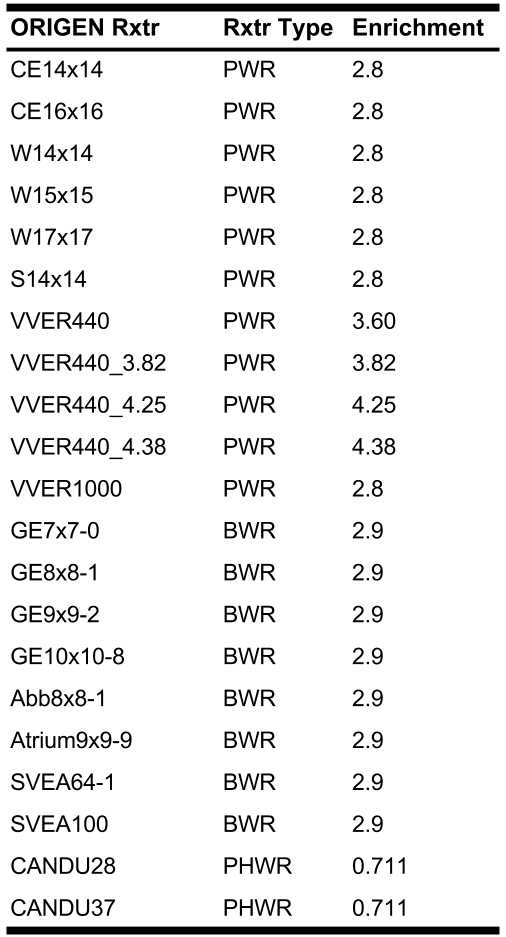
\includegraphics[height=0.7\textheight]{./chapters/demo_method/TrainData.png}
    \caption{Reactor types and uranium-235 enrichment [weight\%].}
    \label{tbl:rxtrtype}
  \end{subtable}
  \begin{subtable}{\linewidth}
    \centering
    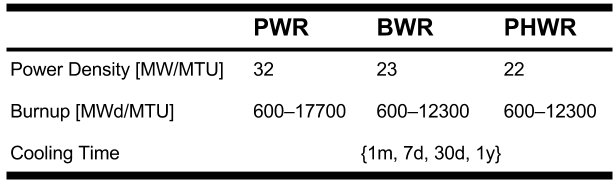
\includegraphics[width=0.7\linewidth]{./chapters/demo_method/TrainData2.png}
    \caption{Simulation space defining reactor parameters and cooling time.}
    \label{tbl:rxtrparam}
  \end{subtable}%
  \caption{Design of the training set space.}
  \label{tbl:train}
\end{table}

It should be noted that many algorithms are developed on an assumption that the
training set will be \gls{i.i.d.}. This is important so that the model does not
overvalue or overfit a certain area in the training space.  A truly
\gls{i.i.d.} training set would go beyond the lower burnups, but this is purely
for demonstration with a single use case in mind.  The training database is
thus constructed by simulating the same training set space as described in Ref.
\cite{dayman_feasibility_2013}, shown in Table \ref{tbl:train}. For each entry 
shown here the simulations included 

While in most machine learning studies the testing set is chosen randomly from
the training set, the previous work used an external one, shown in Table
\ref{tbl:test}.  Although the test set was designed to have values in between
the trained values of burnup, it was chosen systematically. Therefore it was
implemented in this study for comparison, but cross-validation will be used
moving forward. More specifically, using \textit{k}-fold cross-validation is
expected to better indicate the model performance. 

\begin{table}[H]
  \centering
  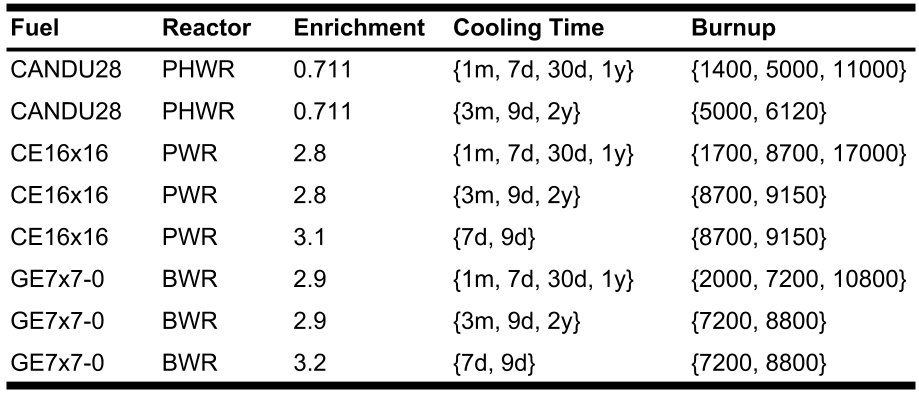
\includegraphics[width=0.95\linewidth]{./chapters/demo_method/TestData.png}
  \caption{Design of the testing set space.}
  \label{tbl:test}
\end{table}

\subsection{Information Reduction}
\label{sec:inforeduc}

Since the overall goal of this project is to determine how much information to
what quality is needed to train a machine-learned model, there will be an 
information reduction manipulation applied to the training data set. This study 
evaluates the impact of randomly introduced error of varying amounts on the 
ability of the algorithms to correctly predict the burnup. 

The three algorithms will be evaluated with error applied to each nuclide
vectors in the training set.  A maximum error is ranging from $0 - 10\%$ is
chosen for each round of training, and a random error within the range of
$[1-E_{max}, 1+E_{max}]$ is applied to each component of the nuclide vector.

However, since error in a nuclide vector is not random, in fact it is
systematic and dependent on a number of known sources of uncertainty, the next
study will introduce error by limiting the nuclides to only those that can be
measured with a gamma spectrometer. This will use the code \gls{GADRAS-DRF}
\cite{gadras} to computationally generate gamma spectra from the nuclide
vectors, and is the next step in the future work. This is discussed in more
detail in Chapter \ref{ch:future}.

